% Chapter 9
\chapter{RoPE in the Window Branch}
\label{ch:rope}

This chapter addresses RQ3. It tests the cause that \cref{ch:xai} found: the window branch without RoPE. The change is one option of v2, \code{window_rope}. All other settings are the settings of Run~1: feature dimension 128, the LoLCATs recipe and bf16. The paper of Lizard writes the window without RoPE. Thus this model is an extension of Lizard, not the reproduction.

\section{Why RoPE in the window, and the predictions}
\label{sec:rope-why}

The branch decomposition gave reference values for Run~1. A conversion of the remaining errors into stage 1 losses gave estimates before the run. The trained output of Run~1 converts to 3.25. The best mix of the two trained branches (G+W) gives 2.96. A window with RoPE alone (WR) gives 2.43. The trained gated branch with a window with RoPE (G+WR) gives 1.20. \Cref{tab:predictions} lists the six predictions and the results.

\begin{table}[ht]
\centering
\small
\caption[Predictions before the \code{window_rope} run and the results]{Predictions before the \code{window_rope} run and the results (project notes, \enquote{RoPE in the window branch}). All six predictions hold.}
\label{tab:predictions}
\begin{tabularx}{\linewidth}{@{}LL@{}}
\toprule
Prediction & Result \\
\midrule
1. The stage 1 loss falls clearly below 3.25, probably below 2.96. & 1.2290. It is also below 2.43, so the trained gated branch adds to the window with RoPE. \\
2. The loss does not reach 1.20, because the gated branch keeps the weight 1. & 1.2290, 2\% above 1.20 \\
3. The relative MSE at positions 0--127 falls clearly from 0.463, but stays above 0. & 0.321 ($-31\%$) \\
4. Layers 0 and 15, and heads 14 and 23 of layer 15, improve most. & Layer 15: 5.3$\times$, layer 0: 3.7$\times$. Heads 14 and 23: 13.7$\times$ and 11.3$\times$. \\
5. $\alpha$ of layer 0 rises above 0.042. & 0.660 \\
6. PIQA and ARC-Easy increase, PIQA by at least 3.2 points. & PIQA +3.9, ARC-Easy +4.3 \\
\bottomrule
\end{tabularx}
\end{table}

\section{What RoPE in the window means for the linearization}
\label{sec:rope-meaning}

RoPE is only in the window branch. The function \code{window_inputs} rotates the queries and keys of the window. The function \code{feature_maps} gets the queries and keys without RoPE. Thus the kernel $\phi(\vq_i)^\top\phi(\vk_t)$ of the gated branch depends only on the content of the tokens.

\textbf{The window branch is not a linear attention.} It is a softmax attention over the last 128 keys and the 4 sinks. Linearization applies only to the gated branch. Thus RoPE in the window does not change the cost or the memory. Each key gets its rotation one time, at its own position, when it goes into the cache. A RoPE score depends only on the distance (\cref{eq:rope}), so the rotated keys in the cache stay valid (\cref{tab:proofs}, P5).

\textbf{Inside the window, the scores are the scores of the teacher.} With RoPE, the window score is $(R_i\vq_i)^\top(R_t\vk_t)/\sqrt{d}$, as in the teacher. Thus for the keys inside the window, the window weights are proportional to the weights of the teacher. Only the denominator differs: it is the sum over the window and the sinks, not over all earlier keys. Without RoPE, the window knows which keys are inside it, but not their order.

\textbf{The two branches get separate tasks.} The window gives the local attention of the teacher. The gated branch must only approximate the part of the teacher output from keys outside the window. Thus the error of the linearization moves to the long range.

\textbf{The gated branch still has no position code.} Its only position information is the decay $\prod \gamma$. In \code{window_rope}, 99.9--100.0\% of the tokens in layers 1--15 have $\gamma > 0.999$. \Cref{fig:gate-decay} shows what this means. If all gates are above 0.999, a token keeps more than $0.999^{128} \approx 0.88$ of its weight after 128 tokens and more than $0.999^{2048} \approx 0.13$ after 2048 tokens. Thus in these layers, the gated branch is almost a mean of the earlier tokens, with weights from the feature similarity. Layer 0 is different: its gate keeps 0.87 of the weight after 128 tokens.

\begin{figure}[ht]
\centering
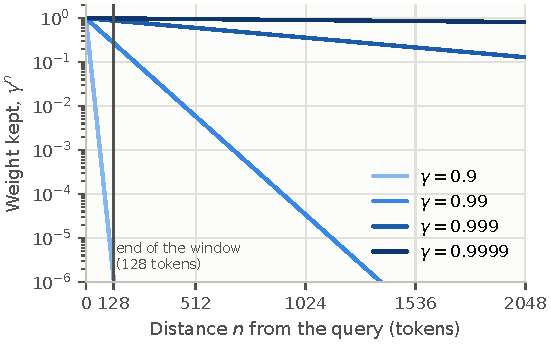
\includegraphics[width=0.66\linewidth]{gate_decay}
\caption[Weight that the gate keeps after $n$ tokens]{Weight $\gamma^n$ that a constant gate keeps after $n$ tokens. In \code{window_rope}, almost all gates of layers 1--15 are above 0.999. Then the gated branch hardly prefers recent tokens.}
\label{fig:gate-decay}
\end{figure}

\Cref{tab:rope-methods} compares the methods. The gated branch could also get RoPE, as in LoLCATs: $\phi(R_i\vq_i)^\top\phi(R_t\vk_t)$. The form stays linear and recurrent. But the Hedgehog map is not linear, so this kernel is not a function of the distance only. The code does not have this option yet.

\begin{table}[ht]
\centering
\small
\caption[Where each method uses RoPE]{Where each method uses RoPE (project notes, document~15 and \enquote{RoPE in the window branch}).}
\label{tab:rope-methods}
\begin{tabularx}{\linewidth}{@{}lLL@{}}
\toprule
Method & Window branch & Linear or gated branch \\
\midrule
LoLCATs & RoPE & RoPE: the feature maps get the queries and keys after RoPE \\
Lizard paper & No RoPE & No RoPE. Position only from the gate. \\
Liger & Paper: no RoPE. Code: RoPE. & No RoPE \\
\code{window_rope} & RoPE & No RoPE. Position only from the gate. \\
\bottomrule
\end{tabularx}
\end{table}

\section{Results after stage 1}
\label{sec:rope-stage1}

\Cref{tab:rope-stage1} gives the scores after stage 1. PIQA and ARC-Easy rise clearly. These are the highest scores of all Lizard stage 1 checkpoints. The loss falls by 62\% and closes 72\% of the gap to the LoLCATs control. But PIQA closes only 25\% of its gap, and ARC-Easy 18\%. The collapse to \enquote{A} on MMLU is mostly gone.

\begin{table}[ht]
\centering
\small
\caption[\code{window_rope} after stage 1]{\code{window_rope} after stage 1 against Run~1 and the LoLCATs control (project notes, \enquote{RoPE in the window branch}). $z$ values with unpaired SEs.}
\label{tab:rope-stage1}
\begin{tabular}{@{}lrrrr@{}}
\toprule
Measure & Run 1 & \code{window_rope} & Difference & LoLCATs control \\
\midrule
Stage 1 loss & 3.2549 & \textbf{1.2290} & $-62\%$ & 0.4442 \\
PIQA & 57.6 $\pm$ 1.2 & \textbf{61.5} $\pm$ 1.1 & +3.9 ($z \approx 2.4$) & 73.5 \\
ARC-Easy & 39.0 $\pm$ 1.0 & \textbf{43.3} $\pm$ 1.0 & +4.3 ($z \approx 3.0$) & 62.8 \\
MMLU subset & 22.5 & 24.6 & +2.1 ($z \approx 0.6$) & 26.0 \\
\enquote{A} on MMLU & 95.4\% & 40.0\% & -- & 19.3\% \\
$\alpha$ of layer 0 & 0.042 & 0.660 & -- & -- \\
\bottomrule
\end{tabular}
\end{table}

\Cref{fig:rope-layer} shows that the MSE falls in every layer, most of all in layers 15 and 0. Heads 14 and 23 of layer 15 now give 4.4\% of the loss, against 21\% in Run~1. For the first time, a Lizard checkpoint has less than 3.0 times the MSE of the control in some layers (10 of 16).

\begin{figure}[ht]
\centering
\includegraphics[width=\linewidth]{window-rope/layer_mse_vs_run1}
\caption[Layer-wise MSE of \code{window_rope} against Run~1]{Layer-wise MSE of \code{window_rope} (orange) against Run~1 (blue). Panel (b) shows the difference. Source: project notes, \enquote{RoPE in the window branch}.}
\label{fig:rope-layer}
\end{figure}

The branch decomposition explains why the accuracy rose less than the loss (\cref{fig:rope-branch}). At positions 0--127, the window with RoPE alone now keeps an error of only 0.048 (Run~1: 0.403). The rest comes from the sinks. But the trained output has an error of 0.321 there, while the best mix of the same two branches has 0.025. Thus at short positions, the \emph{mix} of the branches gives most of the error. The best weight of the gated branch is 0.08 at positions 0--127, 0.65 at positions 128--511 and 0.79 at positions 512--2047. With \code{gla_norm: row}, the gated branch keeps the weight 1 at every position. In the stage 1 loss, 94\% of the positions are above 127. Thus the training sets the mix for long contexts, and the short prompts of PIQA and ARC-Easy get a mix that does not fit them.

\begin{figure}[ht]
\centering
\includegraphics[width=\linewidth]{window-rope/branch_fit_0-127}
\caption[Branch decomposition at positions 0--127]{Branch decomposition at positions 0--127 for Run~1 (left) and \code{window_rope} (right). Each cell is the remaining error after the best fit of a set of branches. In \code{window_rope}, the window W alone is almost exact (light cells), but the trained output (last column) is not. Source: project notes, \enquote{RoPE in the window branch}.}
\label{fig:rope-branch}
\end{figure}

\begin{figure}[ht]
\centering
\includegraphics[width=0.72\linewidth]{window-rope/position_heatmap}
\caption[Relative MSE by layer and position bucket]{Relative MSE by layer and position bucket for Run~1 (left) and \code{window_rope} (right). Short positions now have the largest error, most of all in layers 2 and 3. Source: project notes, \enquote{RoPE in the window branch}.}
\label{fig:position-heatmap}
\end{figure}

\section{Results after stage 2}
\label{sec:rope-stage2}

Stage 2 trained only the LoRA weights, as in Run~2. Its validation loss fell from 1.3432 to 1.2352, against 2.252 for Run~2. \Cref{tab:rope-stage2} gives the scores.

\begin{table}[ht]
\centering
\small
\caption[\code{window_rope} after stage 2]{\code{window_rope} after stage 2 (project notes, \enquote{RoPE in the window branch}, Run~2, and document~7, section~6). Accuracy in \%.}
\label{tab:rope-stage2}
\begin{tabular}{@{}lrrrr@{}}
\toprule
Task & \makecell[r]{First Lizard\\model} & \code{window_rope} & Difference & \makecell[r]{Teacher,\\this harness} \\
\midrule
PIQA & 67.95 $\pm$ 1.09 & \textbf{73.1} $\pm$ 1.0 & +5.1 ($z \approx 3.4$) & 74.4 $\pm$ 1.0 \\
ARC-Easy & 54.8 $\pm$ 1.0 & \textbf{63.8} $\pm$ 1.0 & +9.0 ($z \approx 6.3$) & 65.3 $\pm$ 1.0 \\
MMLU subset & 24.9 & 25.6 & +0.7 & 33.7 \\
MMLU, all questions & 23.3 & \textbf{27.2} $\pm$ 0.4 & +3.9 & 31.7 $\pm$ 0.4 \\
Stage 2 validation loss & 2.252 & 1.235 & -- & -- \\
\bottomrule
\end{tabular}
\end{table}

\begin{figure}[ht]
\centering
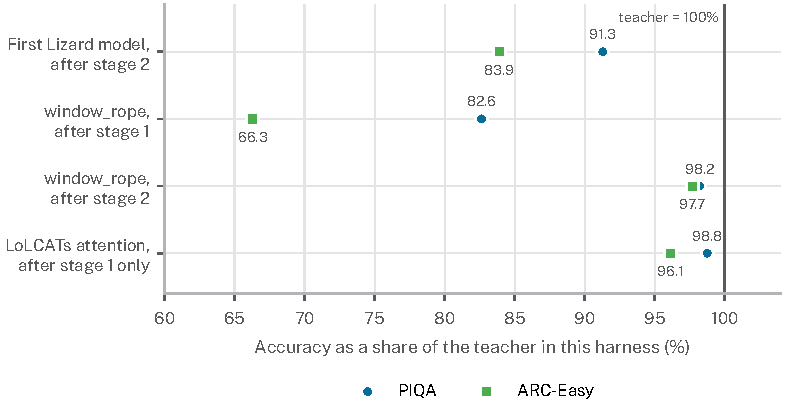
\includegraphics[width=\linewidth]{percent_of_teacher}
\caption[PIQA and ARC-Easy as a share of the teacher]{PIQA and ARC-Easy as a share of the teacher in this harness (74.43 and 65.32). After stage 2, \code{window_rope} reaches 98.2\% and 97.7\%. The LoLCATs control reaches a similar level after stage 1 alone.}
\label{fig:percent}
\end{figure}

\begin{finding}
After stage 2, \code{window_rope} is the best Lizard model of this work. It gets 98.2\% of the teacher on PIQA and 97.7\% on ARC-Easy (\cref{fig:percent}). The differences to the teacher are $-1.4$ points ($z \approx -0.9$) and $-1.5$ points ($z \approx -1.1$), so they are not clear. The gain of stage 1 grows in stage 2: from +3.9 to +5.1 points on PIQA, and from +4.3 to +9.0 points on ARC-Easy.
\end{finding}

\section{The shared denominator does not help}
\label{sec:hybrid}

The mix problem of \cref{sec:rope-stage1} suggested the next step: the shared denominator of LoLCATs (\code{gla_norm: hybrid}). With this option, the share of the gated branch can grow with the position. The run started $\alpha$ at 0.1, as LoLCATs does. \Cref{tab:hybrid} gives the result.

\begin{table}[ht]
\centering
\small
\caption[\code{window_rope} with and without \code{hybrid}]{\code{window_rope} with and without \code{hybrid}, after stage 1 (project notes, \enquote{\code{window_rope} with the shared denominator}).}
\label{tab:hybrid}
\begin{tabular}{@{}lrrr@{}}
\toprule
Measure & \code{window_rope} & with \code{hybrid} & Difference \\
\midrule
Stage 1 loss & \textbf{1.2290} & 1.6172 & +32\% \\
PIQA & \textbf{61.5} & 58.9 & $-2.6$ ($z \approx -1.6$) \\
ARC-Easy & \textbf{43.3} & 36.0 & $-7.3$ ($z \approx -5.1$) \\
MMLU subset & 24.6 & 25.3 & +0.7 \\
Relative MSE, positions 0--127 & 0.321 & \textbf{0.222} & $-31\%$ \\
\bottomrule
\end{tabular}
\end{table}

The gate split the layers into two groups. In 7 layers, the gate stayed open, and the MSE fell at all positions. In layer 0, the MSE fell 5.8 times. In the other 9 layers, the gate closed: $\gamma$ fell below 0.001 for almost all tokens, so the gated branch kept only the current token. These 9 layers lost the long range. Their MSE was 1.8--2.7 times that of \code{window_rope}, and they gave 78\% of the loss. The error at short positions fell, but PIQA and ARC-Easy fell too. Thus \code{window_rope} with \code{row} stayed the best setting.

\section{Table 9 of the paper}
\label{sec:table9}

\Cref{tab:table9} compares \code{window_rope} with Table~9 of the paper. The paper used a newer harness, so only the teacher rows of the same harness give the real gap. ARC-Challenge and HellaSwag ran on 2026-10-11. WinoGrande has no result yet.

\begin{table}[ht]
\centering
\small
\caption[\code{window_rope} against Table 9 of the paper]{\code{window_rope} after stage 2 against Table~9 of the paper. Accuracy in \%. ARC-Challenge, HellaSwag and WinoGrande use \code{acc_norm}, \code{acc_norm} and \code{acc}, as in the paper.}
\label{tab:table9}
\setlength{\tabcolsep}{4pt}
\begin{tabular}{@{}lrrrrrr@{}}
\toprule
Model & PIQA & ARC-e & ARC-c & \makecell[r]{Hella-\\Swag} & \makecell[r]{Wino-\\Grande} & MMLU \\
\midrule
Teacher, this harness & 74.4 & 65.3 & -- & -- & -- & 31.7 \\
\code{window_rope}, this harness & 73.1 & 63.8 & 36.1 & 60.7 & pending & 27.2 \\
\midrule
Teacher, paper & 74.1 & 65.4 & 36.4 & 63.8 & 60.0 & 31.0 \\
LoLCATs, paper & 74.6 & 63.0 & 35.1 & 63.7 & 61.5 & 27.3 \\
Lizard, paper & 74.8 & 65.6 & 36.5 & 64.1 & 59.7 & 29.8 \\
\bottomrule
\end{tabular}
\end{table}

On ARC-Challenge, \code{window_rope} gets 36.1 with \code{acc_norm} (33.2 with \code{acc}). This is within 0.4 points of the paper values for the teacher and for Lizard. On HellaSwag, it gets 60.7 $\pm$ 0.5 with \code{acc_norm} (47.1 with \code{acc}). This is 3.1 points below the teacher of the paper (63.8), a larger gap than on the other short tasks. The teacher of this harness has no value on these tasks yet. If the two harness versions agree here as on PIQA and ARC-Easy, \code{window_rope} keeps approximately 95\% of the teacher on HellaSwag.

\section{MMLU on all questions}
\label{sec:mmlu-full}

The MMLU subset has an SE of 2.6 points. Thus both models also ran on all 14,042 questions (\cref{tab:mmlu-full}).

\begin{table}[ht]
\centering
\small
\caption[MMLU on all questions]{MMLU on all questions, 5-shot (project notes, \enquote{RoPE in the window branch}, findings 15--21).}
\label{tab:mmlu-full}
\begin{tabular}{@{}lrr@{}}
\toprule
Measure & Teacher & \code{window_rope} \\
\midrule
Mean over the subjects & \textbf{31.7} $\pm$ 0.4 & \textbf{27.2} $\pm$ 0.4 \\
Mean over the questions & 31.0 & 26.9 \\
Probability mass of the four letters & 0.999 & 0.975 \\
Confidence (largest letter probability) & 0.342 & 0.354 \\
Entropy over the four letters & 1.904 bits & 1.900 bits \\
\bottomrule
\end{tabular}
\end{table}

\textbf{The model is above chance, but it keeps only one third of the knowledge.} 27.2 is approximately 5.9 SE above 25\%. The first Lizard model was 4.8 SE below. On the same questions, the teacher has 4.2 more points (paired SE 0.44, $z \approx 9.5$). The teacher alone is right on 2,210 questions, and the student alone on 1,625 (McNemar $z \approx 9.5$). The student gets 86\% of the teacher score, but only 33\% of the part of the teacher score above chance: $(27.2 - 25)/(31.7 - 25)$.

\textbf{The student follows the teacher.} When the teacher is right, the student is right on 49.3\% of the questions. When the teacher is wrong, the student is right on only 16.8\%. Without a link between the models, both values would be 26.9\%.

\textbf{The student loses most where the teacher knows most.} \Cref{fig:mmlu-groups} shows the four subject groups. The gap is 2.8 and 2.7 points in STEM and the humanities, where the teacher is near chance. It is 4.7 and 7.2 points in the social sciences and the group \enquote{other}, where the teacher knows more. \Cref{fig:mmlu-subjects} shows the same pattern for the single subjects.

\begin{figure}[ht]
\centering
\begin{minipage}[t]{0.6\linewidth}
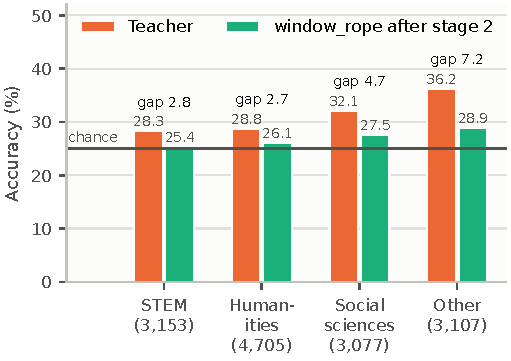
\includegraphics[width=\linewidth]{mmlu_groups}
\caption[MMLU by subject group]{MMLU by subject group, with the number of questions. The values are means over the questions of each group.}
\label{fig:mmlu-groups}
\end{minipage}\hfill
\begin{minipage}[t]{0.37\linewidth}
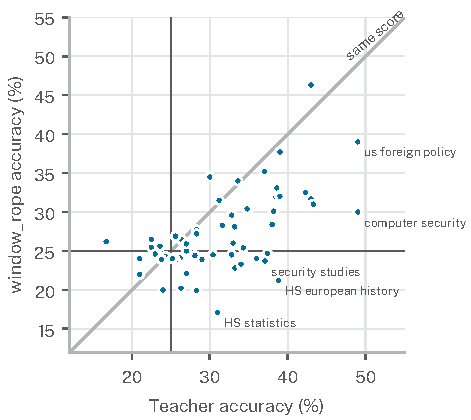
\includegraphics[width=\linewidth]{mmlu_subjects}
\caption[MMLU for each subject]{MMLU for each of the 57 subjects. Points below the diagonal are subjects where the student loses. Data in Appendix~\ref{app:mmlu}.}
\label{fig:mmlu-subjects}
\end{minipage}
\end{figure}

\textbf{The gap does not grow with the prompt length.} In the four quarters of the prompt length, the gap is 5.9, 3.8, 2.4 and 4.5 points. The shortest prompts have the largest gap. The length and the subject are not independent, but this result does not support the idea that the long 5-shot context causes the gap.

\section{Letters and ties on MMLU}
\label{sec:ties}

\Cref{fig:mmlu-letters} shows the letters that the two models select. Both models prefer \enquote{A} and almost never give \enquote{D}. Thus the even spread over the letters is a property of the 1B teacher in this format, not a sign of damage in the student. The gap is in the choice of the right letter.

\begin{figure}[ht]
\centering
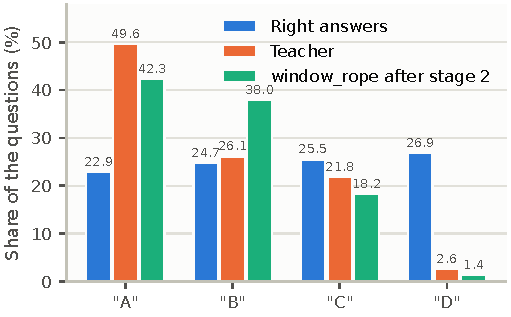
\includegraphics[width=0.66\linewidth]{mmlu_letters}
\caption[Selected letters on all MMLU questions]{Selected letters on all MMLU questions, and the share of each letter among the right answers.}
\label{fig:mmlu-letters}
\end{figure}

The letter log-likelihoods of both models are multiples of 0.125 or 0.25, because the logits are in bf16. Thus ties at the maximum are common: 24.2\% of the teacher answers and 20.5\% of the student answers. In a tie, the harness selects the first letter. Suppose that a random choice breaks each tie. Then the mean over the questions is 31.7 for the teacher (stored 31.0) and 27.0 for the student (stored 26.9). The ties add to the preference for \enquote{A}, but the rare \enquote{D} does not come from the ties.

\begin{finding}
\textbf{RQ3.} RoPE in the window branch closes almost all of the gap on PIQA and ARC-Easy. It does not close the gap on MMLU: 27.2 against 31.7 for the teacher. The shared denominator does not help, because the gate closes in 9 of 16 layers.
\end{finding}
